\section{Preliminaries}\label{sec:preliminaries}

\subsection{Reinforcement learning}\label{sec:preliminaries:rl}

Reinforcement learning (RL) is an approach to automate goal-directed learning~\citep{RLIntroBook}. It relies on two entities that interact with each other: an \textit{environment} that delivers information of its \textit{state}, and an \textit{agent} that using such information learns how to achieve a \textit{goal} in the environment. The interaction is a bilateral communication where the \text{agent} performs \textit{actions} to modify the \textit{state} of the environment, which responds with a numeric \textit{reward} measuring how good the action was to achieve the \textit{goal}. Typically, the sole interest of the agent is to improve its decision-making strategy, known as the \textit{policy}, to maximize the total reward received over the whole interaction trial since this will lead it to the desired goal. More strictly, RL is formalized using finite Markov Decision Processes (MDPs) as in Definition~\ref{def:preliminaries:rl} borrowed from~\cite{RL2}, resulting in the agent-environment interaction illustrated in Figure~\ref{fig:preliminaries:rl}.


\begin{definition}[Reinforcement Learning]
\label{def:preliminaries:rl}
We define a discrete-time finite-horizon discounted MDP $M = (\mathcal{X}, \mathcal{A}, \mathcal{P}, r, \rho_0, \gamma, T)$, in which $\mathcal{X}$ is a state set, $\mathcal{A}$ an action set, $\mathcal{P}: \mathcal{X} \times \mathcal{A} \times \mathcal{X} \mapsto \mathbb{R}_+$ a transition probability distribution, $r: \mathcal{X} \times \mathcal{A} \mapsto [-R_{max}, R_{max}]$ a bounded reward function, $\rho_0 : \mathcal{X} \mapsto \mathbb{R}_+ $ an initial state distribution, $\gamma \in [0,1]$ a discount factor, and $T$ the horizon.
\textsc{Reinforcement learning} typically aims to optimize a stochastic policy $\pi_\theta : \mathcal{X} \times \mathcal{A} \mapsto \mathbb{R}_+$ by maximizing the expected reward, modeled as $\eta(\pi_\theta) = \mathbb{E}_\tau[\sum_{t=0}^{T}{\gamma^tr(x_t, a_t)}]$, where $\tau = (s_0, \alpha_0, ...)$ denotes the whole trajectory, $x_t \in \mathcal{X}$, $x_0 \sim \rho_0(x_0)$, $a_t \in \mathcal{A}$, $a_t \sim \pi_\theta(a_t | x_t)$, and $x_{t+1} \sim \mathcal{P}(x_{t+1}| x_t, a_t)$.

\end{definition}

\begin{figure}[ht]
\begin{center}
\begin{tikzpicture}

% definitions
\tikzstyle{box} = [rectangle, minimum width=2cm, minimum height=0.8cm, text centered, draw=black, fill=gray!0]

% the graph
\node (agent) [box] at (0,0) {\footnotesize Agent};
\node (env) [box, below of=agent, yshift=-1cm] {\footnotesize Environment};

\draw [-{Latex[length=3mm]}] 
    (env) -- +(-3,0) |- node[right, pos=0.25] {\footnotesize $r_t=r(x_t, a_t)$} ($(agent)+(-1, -0.25)$);

\draw [-{Latex[length=3mm]}] 
    ($(env)+(-1.1, 0)$) -- +(-3, 0) |- node[right, pos=0.25] {\footnotesize $x_t$} ($(agent)+(-1, 0.25)$);
    
\draw [-{Latex[length=3mm]}] 
    (agent) -- +(2.5,0) |- node[left, pos=0.25] {\footnotesize $a_t$} (env);

\end{tikzpicture}
\caption{Graphic representation of the reinforcement learning interaction. Every time the agent performs an action $a_t$, the environment modifies its state $x_{t-1}$ to $x_t$, computes the reward $r_t$ and sends both values to the agent, who uses them to optimize its policy.}
\label{fig:preliminaries:rl}
\end{center}
\end{figure}

\subsection{Neural Architecture Search}\label{sec:preliminaries:nas}

Neural Architecture Search (NAS) is the process of automating the design of neural networks. In order to formalize this definition, it is convenient to refer to the survey of~\citet{NASsurvey}, which characterize a NAS work with three variables: the \textit{search space}, the \textit{search strategy}, and the \textit{performance estimation strategy}. Figure~\ref{fig:preliminaries:nas} illustrates the interaction between these variables.

\begin{figure}[ht]
\begin{center}
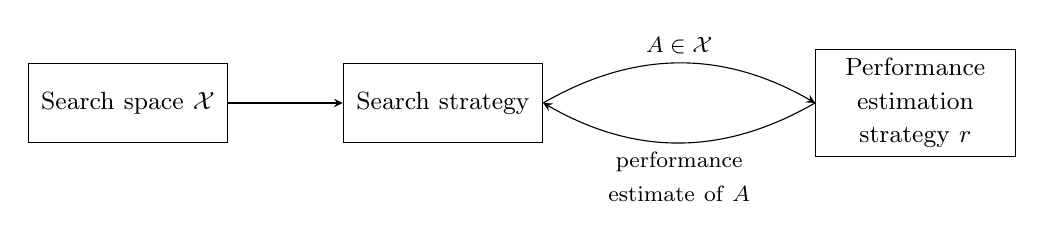
\begin{tikzpicture}

% definitions
\tikzstyle{box} = [rectangle, minimum width=2cm, minimum height=1cm, text width=2.3cm, text centered, draw=black, fill=gray!0]


\tikzstyle{arrow} = [->,>=stealth]


% the graph
\node (ss) [box] at (0,0) {\small Search space $\mathcal{X}$};
\node (st) [box, right of=ss, xshift=3cm] {\small Search strategy};
\node (pss) [box, right of=st, xshift=5cm] {\small Performance estimation strategy $r$};


\draw [arrow] (ss) -- (st);

\draw [arrow] (st.east) to [out=30,in=150] node [above,midway,text centered] {\footnotesize $ A \in \mathcal{X}$ } (pss.west);

\draw [arrow] (pss.west) to [out=210,in=330] node [below,midway, text width=2cm, text centered] {\footnotesize performance estimate of $A$} (st.east);



\end{tikzpicture}
\caption{An illustration of the three NAS variables interacting~\citep{NASsurvey}. At any moment during the search, the \textit{search strategy} samples an architecture $A$ from the \textit{search space} and sends it to the \textit{performance estimation strategy}, which returns the performance estimate. By design, the \textit{search space} and the \textit{performance estimation strategy} are named after the variables in Definition~\ref{def:preliminaries:rl} since they are typically equivalent in NAS within the reinforcement learning setting.}
\label{fig:preliminaries:nas}
\end{center}
\end{figure}

The \textit{search space} is the set of architectures considered in the search process. It is possible to define different spaces by constraining attributes of the networks, such as the maximum depth allowed, the type of layers to use, or the connections permitted between layers. A common abstraction inspired in popular networks is to separate the search spaces in \textit{chain} structures and \textit{multi-branch} structures that can be either \textit{complete} neural networks or \textit{cells} that can be used to build more complex networks, as illustrated in Figure~\ref{fig:preliminaries:ss}.

\begin{figure}[ht]
\begin{center}
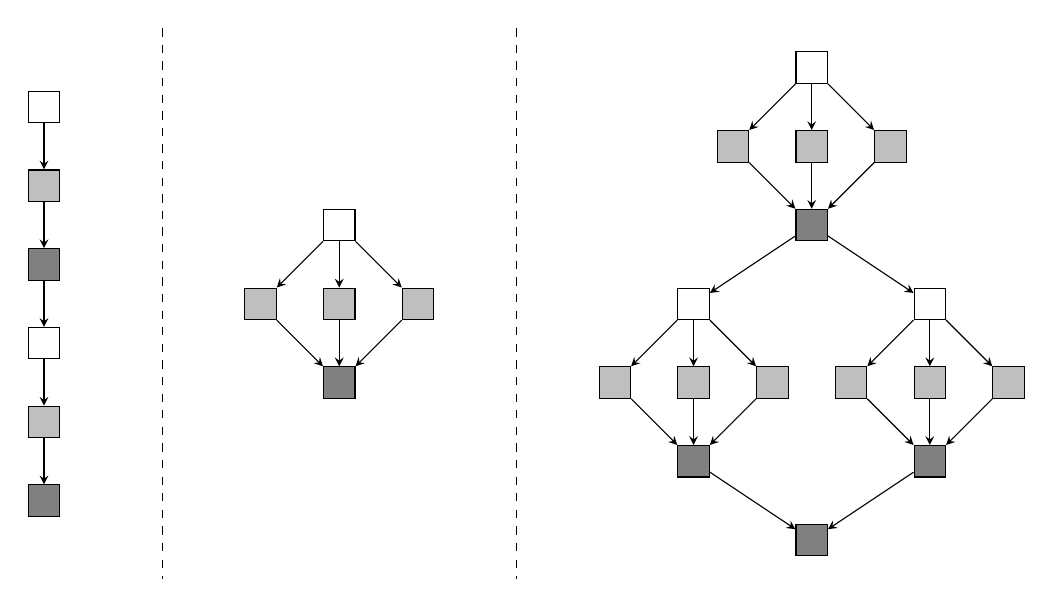
\begin{tikzpicture}

% definitions
\tikzstyle{squareA} = [rectangle, minimum width=0.4cm, minimum height=0.4cm, draw=black, fill=gray!0]

\tikzstyle{squareB} = [rectangle, minimum width=0.4cm, minimum height=0.4cm, draw=black, fill=gray!50]

\tikzstyle{squareC} = [rectangle, minimum width=0.4cm, minimum height=0.4cm, draw=black, fill=gray!100]

\tikzstyle{arrow} = [->,>=stealth]


% chain
\node (aa) [squareA] at (-0.75,-0.5) {};
\node (ab) [squareB, below of=aa] {};
\node (ac) [squareC, below of=ab] {};
\node (ad) [squareA, below of=ac] {};
\node (ae) [squareB, below of=ad] {};
\node (af) [squareC, below of=ae] {};


\draw [arrow] (aa) -- (ab);
\draw [arrow] (ab) -- (ac);
\draw [arrow] (ac) -- (ad);
\draw [arrow] (ad) -- (ae);
\draw [arrow] (ae) -- (af);

\draw[dashed] (0.75, 0.5) -- (0.75, -6.5);


% multi-branch cell
\node (ba) [squareA] at (3,-2) {};
\node (bb) [squareB, below of=ba, left of=ba] {};
\node (bc) [squareB, below of=ba] {};
\node (bd) [squareB, below of=ba, right of=ba] {};
\node (be) [squareC, below of=bc] {};

\draw [arrow] (ba) -- (bb);
\draw [arrow] (ba) -- (bc);
\draw [arrow] (ba) -- (bd);
\draw [arrow] (bb) -- (be);
\draw [arrow] (bc) -- (be);
\draw [arrow] (bd) -- (be);

\draw[dashed] (5.25, 0.5) -- (5.25, -6.5);


% multi-branch stack
\node (ca) [squareA] at (9,0) {};
\node (cb) [squareB, below of=ca, left of=ca] {};
\node (cc) [squareB, below of=ca] {};
\node (cd) [squareB, below of=ca, right of=ca] {};
\node (ce) [squareC, below of=cc] {};

\draw [arrow] (ca) -- (cb);
\draw [arrow] (ca) -- (cc);
\draw [arrow] (ca) -- (cd);
\draw [arrow] (cb) -- (ce);
\draw [arrow] (cc) -- (ce);
\draw [arrow] (cd) -- (ce);

\node (da) [squareA] at (7.5,-3) {};
\node (db) [squareB, below of=da, left of=da] {};
\node (dc) [squareB, below of=da] {};
\node (dd) [squareB, below of=da, right of=da] {};
\node (de) [squareC, below of=dc] {};

\draw [arrow] (da) -- (db);
\draw [arrow] (da) -- (dc);
\draw [arrow] (da) -- (dd);
\draw [arrow] (db) -- (de);
\draw [arrow] (dc) -- (de);
\draw [arrow] (dd) -- (de);

\node (ea) [squareA] at (10.5,-3) {};
\node (eb) [squareB, below of=ea, left of=ea] {};
\node (ec) [squareB, below of=ea] {};
\node (ed) [squareB, below of=ea, right of=ea] {};
\node (ee) [squareC, below of=ec] {};

\draw [arrow] (ea) -- (eb);
\draw [arrow] (ea) -- (ec);
\draw [arrow] (ea) -- (ed);
\draw [arrow] (eb) -- (ee);
\draw [arrow] (ec) -- (ee);
\draw [arrow] (ed) -- (ee);


\draw [arrow] (ce) -- (da);
\draw [arrow] (ce) -- (ea);

\node (f) [squareC, below of=de, right of=de, xshift=0.5cm] {};

\draw [arrow] (de) -- (f);
\draw [arrow] (ee) -- (f);


\end{tikzpicture}
\caption{Examples of networks belonging to different search spaces. On the left, a \textit{chain-structured} network. On the center, a \textit{multi-branch} network. On the right, the same multi-branch structure used as a \textit{cell} repeated multiple times to build a more complex network.}
\label{fig:preliminaries:ss}
\end{center}
\end{figure}


On the other hand, the \textit{search strategy} is simply the algorithm used to perform the search. The choices range from naive approaches such as random search to more sophisticated ones like reinforcement learning~\citep{BakerNAS, ZophNAS1}, evolutionary algorithms~\citep{AmoebaNet}, or gradient descent search~\citep{DARTS}.

Lastly, the \textit{performance estimation strategy} is the function used to measure the goodness of the sampled architectures. Formally, it is a function $R_{D}: \mathcal{X} \mapsto \mathbb{R}$ evaluating an architecture on a dataset $D$. The \textit{vanilla} estimation strategy is the test accuracy after training of a network, but different alternatives are proposed to try delivering an accurate estimate in a short time since expensive training creates a bottleneck in the search process.